\section{何についての数か}

  \subsection{平均が同じ二つの商品}

    食事に行く店を決めたり, 通販で家電を選んだりするとき, まず目に入るのはレビューの星だろう.
    星の平均が4.2の製品と3.1の製品が並んでいたら, とりあえず4.2のほうを開いてみる.
    何十人もの評価を足して割った数を見れば, 一件ずつレビューを読まなくてもだいたいの様子がわかるからだ.

    この計算は, 算数で習った平均そのものである.

    \begin{defi}{平均}{mean}
      $n$個の観測値 $x_1, x_2, \ldots, x_n$ に対し,
      \[
        \bar{x} = \frac{1}{n} \sum_{i=1}^{n} x_i
      \]
      を\textbf{平均}（算術平均）と呼ぶ.
    \end{defi}

    式にすると少し構えてしまうかもしれないが, 要するに全部足してデータの個数で割っているだけだ.
    計算も簡単で, どれほどたくさんのデータがあっても一つの数にまとめられる.

    では, 同じ星4.0の製品が二つ並んでいたらどうだろう.
    レビューの件数も気になるところだが, どちらも同じ20件だったとする.
    こうなると, 星の平均だけを見ていてもどちらを選ぶべきか判断がつかない.

    しかたがないので, 4.0という計算のもとになった20件の評価そのものを確認してみよう.
    商品Bについた20件を, 投稿された順に並べてみる.

    \begin{center}
      5, 5, 1, 5, 5, 5, 1, 5, 5, 5, 5, 1, 5, 1, 5, 5, 5, 5, 1, 5
    \end{center}

    これを見てすぐに気づくのは, 5と1しか並んでいないことだ.
    平均は4.0なのに, 4点をつけた人は一人もいない.

    一方の商品Aの20件は次のようになっている.

    \begin{center}
      3, 4, 5, 4, 4, 3, 4, 5, 4, 3, 4, 4, 5, 3, 4, 5, 4, 3, 4, 5
    \end{center}

    こちらは3と4と5が混ざっていて, 4点が多そうだ.
    どちらの商品も, 20件の数字を全部足して20で割ればきっちり4.0になる.
    しかし, 列を眺めただけでは正確に何点が何件あるのかまでは数えにくい.

  \subsection{点数ごとに数え直す}

    そこで, 点数ごとに何件あるのかを数えてみる.
    1点が何件, 2点が何件, と数え直して, 横軸に点数, 縦軸に件数を取って棒の高さで表してみる.
    \cref{fig:ch02-ab}がその図だ.

    % 図のデータ: 仮. 要作成
    \begin{figure}[htbp]
      \centering
      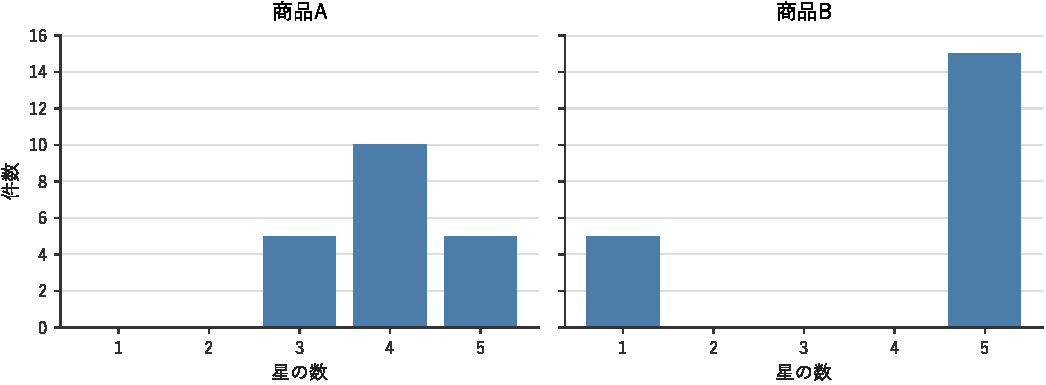
\includegraphics[width=\linewidth]{../figures/output/ch02_ab.pdf}
      \caption{商品Aと商品Bのレビュー20件を, 点数ごとに数えた図. 横軸は星の数, 縦軸は件数. 二つの図で軸をそろえてある.}
      \label{fig:ch02-ab}
    \end{figure}

    こうして並べてみると, 二つの違いがはっきりと見える.
    商品Aは4点が10件あって, その両隣の3点と5点が5件ずつある. 4点を中心にきれいに固まっている.
    これに対して商品Bは, 5点が15件もある一方で, 1点も5件ある. あいだの2点, 3点, 4点は文字どおりゼロだ.

    もちろん, 平均の計算を間違えたわけではない.
    5点が15件（計75点）と1点が5件（計5点）を足せば80点で, 20で割ればたしかに4.0になる.
    ただ, 4.0というのは全員の点数を均等にならした値であって, 一人ひとりの満足度を表しているわけではない.
    商品Bを買った20人のうち5人は, 最低の1点をつけて腹を立てている.

    平均は集まり全体を一つの値で代表させるための数であって, 個別のデータそのものではない.
    「一世帯あたりの子供の数は平均1.6人」と言われても, 実際に1.6人の子供がいる家はどこにもないのと同じことだ.

    このように, 点数ごとに区切って件数を数え上げ, 棒の高さで表した図を\textbf{ヒストグラム}と呼ぶ.
    棒が受け持つ区切りを\textbf{階級}, そこに入ったデータの数を\textbf{度数}という.
    そして, データがどのあたりに多く集まり, どこに少ないのかという全体の姿を, データの\textbf{分布}と呼ぶ.

  \subsection{同じ評価から別の数を出す}

    ヒストグラムを描いてみれば, AとBがまったく別物であることは一目瞭然だ.
    とはいえ, 商品をいくつも比較したいときに, いちいちすべてのレビューを数え直して図を描くのも骨が折れる.
    できれば図を描く手間をかけずに, 平均とは別の数を使ってこの違いを捉えられないだろうか.

    何を知りたいかによって, 計算すべき数は変わってくる.
    たとえば, データを順番に並べたときに, ちょうど真ん中にいる人が何点をつけたかを知りたいとしよう.
    そう思うなら, 20件の点数を小さい順に並べて, 真ん中の値を取り出せばよい.

    \begin{defi}{中央値}{median}
      観測値を小さい順に並べたとき, ちょうど真ん中に来る値を\textbf{中央値}と呼ぶ.
      $n$ が奇数なら $\frac{n+1}{2}$ 番目の値,
      $n$ が偶数なら $\frac{n}{2}$ 番目と $\frac{n}{2}+1$ 番目の値の平均とする.
    \end{defi}

    商品Bの20件を小さい順に並べると, 最初の5件は1点だが, 6件目からはすべて5点になる.
    真ん中にあたる10番目も11番目も5点なので, 中央値は5だ.
    商品Aを小さい順に並べると, 10番目も11番目も4点なので中央値は4になる.
    平均はどちらも同じ4.0だったのに, 真ん中の人がつけた点数は商品Bのほうが高い.

    もう一つ, 図を見ていて気になるのは, 点数の散らばり具合の違いだ.
    商品Aはみんなの評価が4点のまわりにぎゅっと集まっているが, 商品Bは1点と5点に極端に割れている.
    この平均からの離れ具合も, なんとか一つの数にしてみたい.

    データのばらつきを捉えるにはどうすればいいだろうか.
    それぞれのデータが平均からどれくらい離れているかを計算して, 全部足してみればよさそうに思える.
    ところが商品Bで実際にやってみると, 5点の15件は平均の4.0より1大きく, 1点の5件は3小さい.
    これらを足し合わせると, $1 \times 15 + (-3) \times 5 = 0$ となってきれいに消えてしまう.
    商品Aでも同じで, 差の合計はゼロになる.
    平均より大きい値と小さい値が互いに打ち消しあってしまうため, どんなデータであっても単に足すだけでは必ず合計がゼロになってしまうからだ.

    そこで, 差を二乗してから足し合わせることにする.

    \begin{defi}{分散}{variance}
      $n$個の観測値 $x_1, x_2, \ldots, x_n$ とその平均 $\bar{x}$ に対し,
      \[
        s^2 = \frac{1}{n} \sum_{i=1}^{n} (x_i - \bar{x})^2
      \]
      を\textbf{分散}と呼ぶ.
    \end{defi}

    $(x_i - \bar{x})$ でそれぞれのデータが平均からどれだけずれているかを見て, 二乗したものを全部足し, 最後にデータの個数 $n$ で割る.
    データ全体の合計のままでは件数が違う集まりを比べられないので, $n$ で割って1件あたりの大きさに均しているわけだ.

    なぜ二乗するのかと不思議に思うかもしれない.
    符号の打ち消しを防ぐだけなら, 差の絶対値を取って足すだけでもよさそうだ.
    わざわざ二乗するのは, 平均から大きく離れた値をより重く数えるためでもある.
    商品Bの1点は平均から3離れているので, 二乗すると9として計算に入る.
    1しか離れていない5点は, 二乗しても1のままだ.
    つまり, 1点をつけた1人分のずれは, 5点をつけた1人分の9倍もの重みを持って分散を押し上げる.
    分散を見れば, 平均から遠く離れた極端な評価がどれくらい混ざっているかが分かる.

    ただ, 分散には単位の問題がある.
    差を二乗して足しているため, 分散の単位は元のデータの二乗になってしまう.
    たとえば金額のデータなら単位が「$\text{円}^2$」になってしまい, 直感的にどれくらい散らばっているのかがわかりにくい.
    そこで, 分散の正の平方根を取って単位を元のデータと揃えたものを使い, これを標準偏差と呼ぶ.

    \begin{defi}{標準偏差}{stddev}
      分散の正の平方根
      \[
        s = \sqrt{s^2}
      \]
      を\textbf{標準偏差}と呼ぶ.
    \end{defi}

    実際に計算してみると, 商品Aの標準偏差はおよそ0.71, 商品Bはおよそ1.73になる.
    商品Bのほうが倍以上も大きい値だ.

    これで商品Bについて, 平均4.0, 中央値5, 標準偏差1.73という三つの数が手に入った.
    どの計算も間違っていないし, それぞれ別のことに答えている.
    ただし, どれも20件のデータを一つの数にまとめた結果であって, 元の内訳をそのまま持っているわけではない.
    商品Bに4点をつけた人が一人もいなかったという事実は, 20件の数字を自分の目で並べて確認したからわかったのであって, この三つの数字のどこにも直接書かれているわけではない.

  \subsection{何を同じとみなすかを先に決める}

    平均, 中央値, 標準偏差は, どれも手元にある20件のデータから一定の計算手順に従って導き出された数だ.
    ここで, こうした数全体を指す言葉を定義しておこう.

    \begin{defi}{統計量}{stat}
      $n$個の観測値 $x_1, x_2, \ldots, x_n$ から計算される数を\textbf{統計量}と呼ぶ.
    \end{defi}

    観測値から計算される数, というのは, データが決まれば誰が計算しても必ず同じ値になるということだ.
    同じ20件のデータを使えば, 計算する人が違っても平均は4.0になるし, 中央値も標準偏差も同じ値になる.
    つまり統計量とは, 単なる個別の数値というよりも, 「観測値を放り込むと決まったルールで一つの数を返してくれる仕組み」のことだと言ってもよい.
    「平均」や「中央値」という言葉も, その仕組みにつけられた名前にほかならない.

    統計量にいくつもの種類があるのは, 知りたいことが一つではないからだ.
    どの統計量を計算するかを決めるということは, データのどこに目をつぶり, どこを同じとみなすかをあらかじめ決めることでもある.
    そうして同じとみなしたうえで残った違いだけが, 統計量の値として手元に残る.

    たとえば図形の面積で考えてみる.
    正方形と細長い長方形で, 面積がまったく同じになることはいくらでもある.
    面積という数は, 図形がどんな形をしているかという違いをすべて無視して, 広さの違いだけを取り出したものだ.
    だから, 面積が同じだからといって同じ形をしているとは言えない.

    平均もまったく同じことをしている.
    誰が何点をつけたかという個別の内訳をすべて同じとみなして, 全体をならしたときの水準だけを取り出している.
    だから, 平均が同じ4.0であっても, その内訳が同じだとは限らないのだ.

    中央値は, 順に並べたときの真ん中の位置だけを取り出して, 端のデータがどれほど極端な値になっているかは無視する数だ.
    Aの4やBの5という値は, 10番目と11番目に並んだ評価だけで決まっている.
    もし商品Bの1点の5件がすべて2点に上がったとしても, 10番目と11番目は5点のままなので, 中央値は5からびくともしない.

    標準偏差は, 平均からの離れ具合だけを取り出す数であり, 一人ひとりが具体的に何点をつけたかという水準そのものは残さない.
    商品Aでは平均から1離れた人が10人, 離れていない人が10人いて, 標準偏差は0.71になった.
    商品Bで1.73まで大きくなったのは, 5人もの人が平均から3も離れていたからだ.
    ここで, 商品Bの点数をそっくり入れ替えて, 1点が15件, 5点が5件という商品を作ってみたとしよう.
    平均は4.0から2.0へと大幅に下がるが, 平均からの離れ具合の内訳は変わらないため, 標準偏差は1.73のまま変わらない.

    前の章で見たじゃんけんの例でも, まったく同じことが起きていた.
    最初に出てきた 35 : 32 : 33 という手の出現割合は, 誰がどの順番で手を出したかをすべて同じとみなして, 出された手の比率だけを残した数だった.
    だから, 直前に出された手によって次に出る手がどう変わるのかは, その比率を見ているだけではわからない.
    そこで直前の手と次の手の組み合わせに注目して数え直してみると, 直前と同じ手を続けて出す割合は23\%しかなかった.

    また, 評価が星5つの商品があったとしても, それをつけたのがたった1人だけなら, その星5つをそのまま信じるのはためらわれる.
    しかし平均にせよ中央値にせよ標準偏差にせよ, 元のデータが1件しかなくても, 20件あっても, 計算の手順に従って淡々と一つの数を弾き出してしまう.
    「たった1人の評価だから心もとない」という不安は, 計算された統計量そのものには現れてこないのだ.

  \subsection{典型的な一本はどれくらい見られているか}

    ある動画配信サービスに, 邦画が80本あるとしよう.
    どの作品についても, 公開後30日間にどれくらい再生されたかという視聴回数が記録されているとする.
    （なお, このデータは本書のために用意した架空のものであり, 実際の配信サービスの数値ではない.）

    ここで, 知りたいことを一つはっきりさせておく.
    「典型的な1本の映画は, だいたいどれくらい見られているのだろうか」という疑問だ.

    まず, 80本の視聴回数の平均を計算してみると, およそ $209.4$ 万回になる.
    では中央値はどうだろうか. 小さい順に並べて真ん中を取ってみると, $107.1$ 万回だった.
    中央値は平均の半分ほどしかない.

    同じような現象は, 身近な年収のデータでもよく見られる.
    日本の平均年収はおよそ460万円だと言われているが\footnote{%
    国税庁「令和5年分民間給与実態統計調査」による. 1年を通じて勤務した給与所得者の平均給与が460万円. 中央値は同調査では公表されていないが, 給与階級別の分布から400万円前後と読み取れる.},
    中央値を取ると400万円前後になり, 実際には平均以下の年収の人のほうが多数派を占める.
    一部の飛び抜けて高い収入を得ている人たちが, 全体の平均をぐっと引き上げているからだ.
    映画の視聴回数でもまったく同じことが起きていて, 桁外れにヒットしたごく少数の作品が, 平均の数値を押し上げているのである.

    だからといって, 平均という計算が間違っているわけではない.
    80本の映画の再生回数の総計をもとに, 「作品1本あたりにならすとどれくらいになるか」を知りたいのであれば, 全部の視聴回数を足して80で割った平均こそがふさわしい数になる.
    大ヒット作の視聴回数も, サービス全体の総再生回数には現に入っているからだ.
    しかし, 「ごくありふれた典型的な1本がどれくらい見られているか」を知りたいのであれば, 一部の極端な値に引きずられない中央値のほうが実感に近くなる.
    何を知りたいかによって, 役に立つ統計量は異なるのだ.

    ついでに散らばり具合も確認しておこう.
    標準偏差を計算してみると約 $239.3$ 万回となり, 平均の値そのものと同じくらい大きな数字になる.
    標準偏差は平均から離れるほど二乗して大きく数えるため, 桁違いに再生された数本の映画が, この数値をここまで跳ね上げているわけだ.

    この80本のデータについても, 図を描いて全体の姿を確かめてみよう.
    星の評価と違って, 視聴回数は値の種類が多すぎて, 値ごとに数えると棒が一本ずつバラバラに立ってしまう.
    そこで, 視聴回数をいくつかの区間に区切り, それぞれの区間に何本の映画が入るかを数えてヒストグラムにしてみる.
    \cref{fig:ch02-views}がその図である.

    % 図のデータ: 仮. 要作成
    \begin{figure}[htbp]
      \centering
      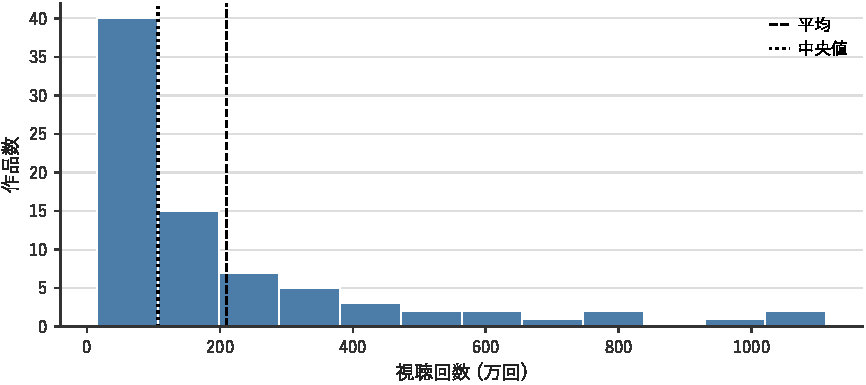
\includegraphics[width=0.85\linewidth]{../figures/output/ch02_views.pdf}
      \caption{映画80本の公開後30日間の視聴回数のヒストグラム. 横軸は視聴回数 (万回), 縦軸は作品の本数.}
      \label{fig:ch02-views}
    \end{figure}

    図を見ると, 左側の低い視聴回数のところに大きな山があり, そこから右側へ向かって細く長く裾が伸びている.
    大半の作品は左側の低い山に集まっていて, ごく一部の作品だけが右側の遠いところまで突き抜けている.
    平均の $209.4$ 万回という値は, この右に長く伸びた裾の大ヒット作に強く引っ張られて, 山の頂上よりもずいぶん右側にある.

  \subsection{手元にある分しか数えていない}

    この80本について計算した平均が $209.4$ 万回であることには, 何の疑いもない.
    80個の数値を電卓に入れて足し算し, 80で割れば, 誰が計算しても正確にこの数になる.

    しかし, この計算結果は「この動画配信サービスにある映画全般が, だいたいどれくらい見られているか」という疑問にまで答えてくれているだろうか.
    典型的な1本の姿を知りたいという問題なら, 平均ではなく中央値を見れば解決した.
    だが, この配信サービスで配信されている映画は, 全部で80本きりではないはずだ.
    手元にない残りの作品がどうなっているのかは, 手元にある80本をどう計算してもわからない.
    どの数を計算するかの問題ではなく, そもそも手元で数えた対象が「その80本」で途切れてしまっているからだ.

    最初に取り上げた商品のレビューを思い出してほしい.
    商品Bについていた20件のレビューは, その商品を買ったすべての人たちの声ではない.
    商品を買った人のうち, たまたまレビューを書き残してくれた20人分の記録にすぎないのだ.
    もし別の20人がレビューを書いていたとしたら, 平均が4.0になったとは限らない.
    評価が星5つであっても1人きりの意見なら信用しきれなかったのも, これと同じことだ.
    その1人がたまたま大満足した人だっただけで, 別の人なら星1つをつけていたかもしれないのである.

    映画の80本についてもまったく同じことが言える.
    いま手元にある80本の平均はたしかに $209.4$ 万回だった.
    しかし, もし別の80本を集めてきて同じように計算していたとしたら, この平均値は一体いくつになっていただろうか.

  \subsection{平均と期待値}

    ここで, 平均という計算と, 確率論で学んだ「期待値」とのつながりを整理しておこう.
    手元にある $n$ 個のデータからどれでも同じ確率で1つを選ぶとすれば, その選ばれた値の期待値は, データの平均とぴったり一致する.

    \begin{prop}{平均と期待値}{mean-expectation}
      重複を許して並べた $n$ 個の値 $x_1, x_2, \ldots, x_n$ からなる集まりから1つをランダムに取り出すとき, その値を確率変数 $X$ とする.
      このとき $X$ の期待値は
      \[
        E[X] = \frac{1}{n} \sum_{i=1}^{n} x_i = \bar{x}
      \]
      に等しい.
    \end{prop}

    詳しい証明は巻末の付録に譲る.

% 以下3つの図はコラム本体で参照するが, tcolorbox の中には float を置けないため, mybox の直前で宣言している.

% 図のデータ: 仮. 要作成
\begin{figure}[htbp]
  \centering
  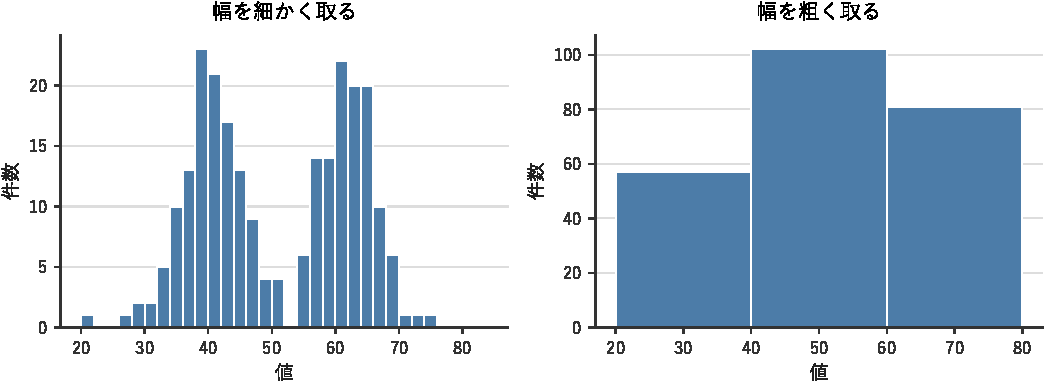
\includegraphics[width=\linewidth]{../figures/output/ch02_col_width.pdf}
  \caption{あるデータを二通りの階級の幅で描いたヒストグラム. 左は幅を細かく, 右は幅を粗く取っている.}
  \label{fig:ch02-col-width}
\end{figure}

% 図のデータ: 仮. 要作成
\begin{figure}[htbp]
  \centering
  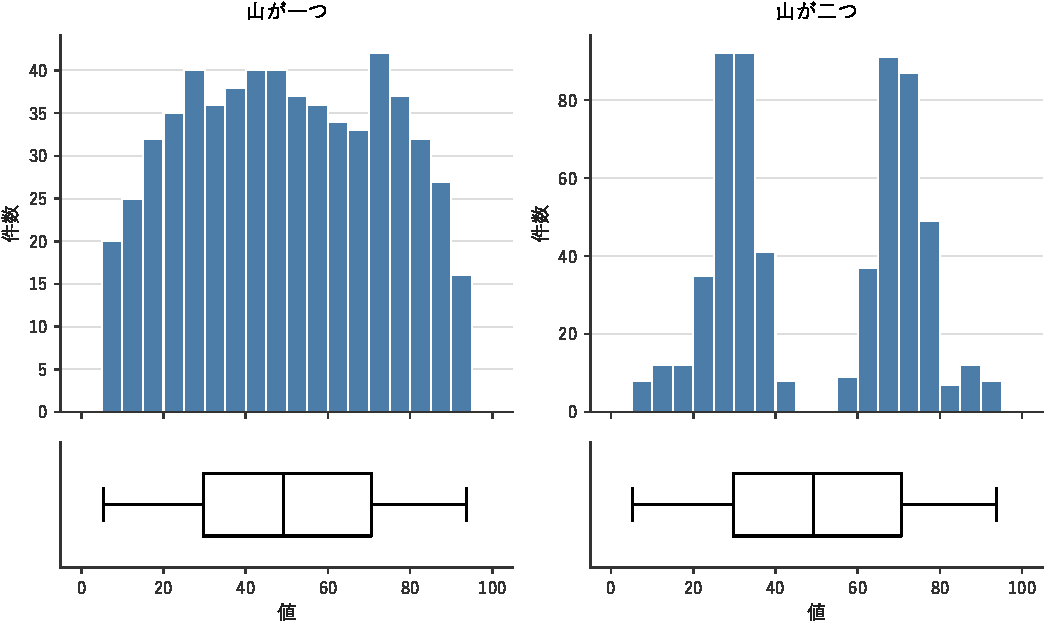
\includegraphics[width=\linewidth]{../figures/output/ch02_col_box.pdf}
  \caption{山が一つのデータと山が二つのデータを, ヒストグラム（上）と箱ひげ図（下）で描いたもの.}
  \label{fig:ch02-col-box}
\end{figure}

% 図のデータ: 仮. 要作成
\begin{figure}[htbp]
  \centering
  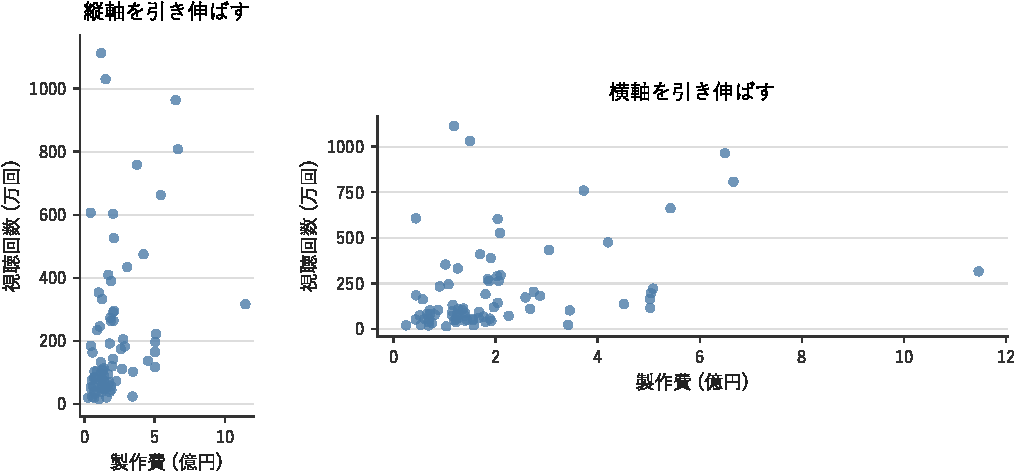
\includegraphics[width=\linewidth]{../figures/output/ch02_col_axis.pdf}
  \caption{同じ点を打った散布図を, 軸の縦横比だけ変えて並べたもの. 横軸は製作費 (億円), 縦軸は視聴回数 (万回).}
  \label{fig:ch02-col-axis}
\end{figure}

\begin{mybox}{数字を変えずに図を変える}

  \subsubsection*{階級の幅}

    ヒストグラムを描くときにデータをどのような幅で区切るかは, あらかじめ決まっているわけではなく, 描く人が自分で決めている.
    まったく同じ一つのデータを, 区切る幅を変えて二通りに描き分けてみたのが\cref{fig:ch02-col-width}だ.

    左側の細かく区切った図では山が二つ並んでいるように見えるが, 右側の粗く区切った図では一つのなだらかな山にまとまっている.
    元の数字は一つも変えていない. 変えたのは階級の幅だけだ.

    幅を細かくしすぎると, たまたま生じたわずかな偏りまでまるで意味のある山のように見えてしまう.
    逆に幅を粗くしすぎると, 全体の形は滑らかになるものの, 本当に二つに分かれていた特徴的な山まで一つにつぶれて見落とされてしまう.
    どちらか一方だけが絶対に正しい図だということはない.
    だからこそ, 一枚のヒストグラムだけを見て早合点してしまわないほうがよいのだ.
    いくつかの異なる幅で図を描いてみれば, どの幅でも共通して現れる特徴と, 区切り方によってたまたま現れた見かけの特徴とを見分けられるようになる.

  \subsubsection*{一番高い棒は何が多いのか}

    データの中で最も頻繁に現れる値には, 最頻値という名前がついている.

    \begin{defi}[unbreakable]{最頻値}{mode}
      観測値の中で最も頻繁に出現する値を\textbf{最頻値}と呼ぶ.
      最頻値は複数存在することもある.
    \end{defi}

    商品AやBのように点数そのものを数えた図であれば, 最も高い棒の点数がそのまま最頻値になる.
    商品Aなら4点, 商品Bなら5点だ.

    しかし, 映画の視聴回数のヒストグラムでは話が変わってくる.
    区間ごとにまとめて数えているため, 一番高い棒が示しているのは「その区間に入った映画の本数が最も多い」ということだけであって, その区間の中の具体的にどの値が一番多いのかまではわからない.
    しかも, 階級の区切り方を変えてしまえば, 最も高い棒が立つ位置そのものが左右に動いてしまうことすらある.

    なお, ヒストグラムの横軸は点数や視聴回数のように数字の大小順に並んでいるため, 棒の並び順を勝手に入れ替えることはできない.
    これに対して, 出身地や血液型のように順序のない項目を横軸に並べたものは棒グラフと呼ばれ, こちらは並び順を自由に入れ替えても図の意味は変わらない.
    見た目はよく似ていても, 横軸に並べているものが違う.

  \subsubsection*{五つの数に切り詰める}

    中央値は, データを小さい順に並べたときにちょうど真ん中に来る値だった.
    同じ考え方を使って, 真ん中以外の位置にある値を取り出すこともできる.

    \begin{defi}[unbreakable]{四分位数と四分位範囲}{iqr}
      観測値を小さい順に並べたとき, 下から $25\%$ の位置にある値を\textbf{第1四分位数} $Q_1$,
      下から $50\%$ の位置にある値を\textbf{第2四分位数} $Q_2$（中央値と一致する）,
      下から $75\%$ の位置にある値を\textbf{第3四分位数} $Q_3$ と呼ぶ.
      位置がちょうど何番目かに当たらないときは, 前後の観測値のあいだを, 位置の端数に応じて按分した値を使う.
      $Q_1, Q_2, Q_3$ をまとめて\textbf{四分位数}と呼ぶ.
      $Q_1$ と $Q_3$ の差
      \[
        \mathrm{IQR} = Q_3 - Q_1
      \]
      を\textbf{四分位範囲}（interquartile range）と呼ぶ.
    \end{defi}

    $Q_1$ から $Q_3$ までの区間には, データを順に並べたときの真ん中の $50\%$ 分のデータがすっぽり収まっている.
    四分位範囲は, その範囲の広さを表す数値だ.
    データの中央半分が狭い範囲に密集しているのか, それとも広く散らばっているのかを表している.

    この $Q_1$, $Q_2$, $Q_3$ と, データ全体の最小値と最大値を一つの図形にまとめたものが箱ひげ図だ.
    箱の中央に引かれた線が中央値で, 箱の両端が $Q_1$ と $Q_3$ を示し, 箱の長さが四分位範囲を表す.
    そして箱の両端から伸びるひげの端点が, 一番小さい値と一番大きい値を表している.

    箱ひげ図を使うとデータ全体がコンパクトな記号にまとまるため, たくさんのグループを横に並べて比較するときに重宝する.
    たとえば映画をジャンルごとに分けて並べれば, それぞれの中央値の高さや散らばりの大きさを一目で比べることができる.
    ヒストグラムを何枚も並べて見比べるよりもはるかに手軽だ.

    ただし, 箱ひげ図は中央値, $Q_1$, $Q_3$, そして両端の最小値と最大値という, たった五つの数だけを使って描かれていることには注意がいる.
    \cref{fig:ch02-col-box}を見てほしい.
    ヒストグラムで見れば一方は山が一つ, もう一方は山が二つに割れていて明らかに形が違うのに, 箱ひげ図にしてしまうとどちらもほぼ同じ形になってしまう.
    箱の中央に線があるからといって, そこにデータが一番たくさん集まっているとは限らないのだ.

    五つの数しか使っていないからこそ並べて比べやすいのだが, 逆に五つの数しか使っていないからこそ, データの重要な山や谷の形が消えてしまうのである.

  \subsubsection*{軸を引き伸ばす}

    二つの数量の関係を調べたいときは, データを1点ずつ平面に打っていく.
    横軸に製作費, 縦軸に視聴回数を取れば, 1本の映画は座標平面上の1個の点になる.
    こうしてすべての映画を点で打った図を散布図と呼ぶ.

    \cref{fig:ch02-col-axis}にある二枚の散布図は, まったく同じデータを打ったものだが, グラフの縦横の比率だけを変えてある.
    縦軸を引き伸ばすとデータは急勾配の右上がりに見え, 逆に横軸を引き伸ばすとごく緩やかな傾きに見える.

    階級の幅を変えたときは, 少なくともまとめ方の数え直しは行っていた.
    だが散布図の縦横比を変えるときは, 数え直しすらしていない. 製作費と視聴回数の数字は少しも動かしていないのだ.
    それでも, 目から入ってくる印象はまるで違ったものになってしまう.

  \subsubsection*{描く前に決まっていること}

    数字は一つも書き換えていないのに, 図のまとめ方を変えるだけで見えるものが何度も入れ替わった.
    区切りの幅, 一番高い棒の意味, 五つの数への切り詰め, そしてグラフの縦横比.
    元データそのものは何も変わっていないのに, 図の上ではまったく違う印象が現れてくる.

    図というのは, データをありのままに写し取ったものではない.
    どこで区切り, どの比率で軸を取るかという判断が入って, はじめて一枚の図になる.
    そしてこれは, 統計量という数についても同じことだ.
    何を知るために計算するのかをあらかじめ決めてはじめて, その数で何が言えるのかが決まる.
    決めるのは, データではなく, 自分が何を知りたいかのほうだ.
\end{mybox}
